\chapter{Results: reproduction and the question of criticality}
\label{ch:results}

\newcommand{\resoffMeanG}{1.6}
\newcommand{\ressumOursG}{1.01}
\newcommand{\ressumTheirsG}{0.21}
\newcommand{\resoffMeanBC}{1.6}
\newcommand{\ressumOursBC}{1.00}
\newcommand{\ressumTheirsBC}{0.20}
\newcommand{\resMstarExp}{0.95}
\newcommand{\restauEllG}{1.96}
\newcommand{\reserrEllG}{0.01}
\newcommand{\restauEllI}{1.92}
\newcommand{\reserrEllI}{0.00}
\newcommand{\restauEllBC}{1.91}
\newcommand{\reserrEllBC}{0.00}
\newcommand{\restauEllBG}{1.88}
\newcommand{\reserrEllBG}{0.00}
\newcommand{\restauEllCE}{1.87}
\newcommand{\reserrEllCE}{0.01}
\newcommand{\reslenLongA}{4008}
\newcommand{\reslenLongB}{2000}
\newcommand{\reslenLongC}{2000}
\newcommand{\reslenLongD}{2001}
\newcommand{\reslenLongE}{2010}


This chapter collects the results on the Burridge--Knopoff model itself. \Cref{sec:res-1991} completes the comparison with Carlson,
Langer, Shaw and Tang (1991) begun in Chapter~\ref{ch:mapping}, including a discrepancy in the normalisation of their figures.
\Cref{sec:res-sigma,sec:res-ell} address the question of whether the model is critical, by varying the friction drop $\sigma$ (which
Carlson \emph{et al.} identify as the critical parameter) and the stiffness $\ell$ (which controls the approach to the continuum limit).
\Cref{sec:res-1989} reproduces the 1989 study of Carlson and Langer, and \cref{sec:res-summary} summarises what has been learned. All
simulations use the programs of Chapter~\ref{ch:numerics}, and all distributions are normalised per unit length and per unit plate
displacement (\cref{sec:bk-stats}).

% ======================================================================
\section{The 1991 model}
\label{sec:res-1991}

\subsection{Shape and exponents}

Chapter~\ref{ch:mapping} showed that our simulations reproduce the features of the size distributions of Carlson \emph{et al.}: peaks of
one- and few-block events, a scaling region of localized events, a minimum near $M=\xi$, a rising branch of delocalized events and a sharp
upper cutoff (\cref{fig:compare,fig:bk-effective}). The exponents of the scaling region agree with theirs: $b = 0.96$, $0.92$ and $0.91$ for
$\ell = 6$, 8 and 12 at $\alpha = 3$ (theirs: $0.92$), and $b\approx0.36$--$0.40$ for $\alpha = 1$ (theirs: $0.35$). The positions of the
minimum and of the peak of delocalized events agree with their Fig.~3 to within a few tenths in $\ln(M/\xi)$.

\subsection{Normalisation}

There is, however, a difference in the \emph{height} of the distributions. \Cref{fig:normalisation} compares our results with values read off
Fig.~3 of Carlson \emph{et al.} at three landmarks: a point in the scaling region, the minimum, and the peak of delocalized events. For both
$\ell = 6$ and $\ell = 12$ their curves lie below ours by an almost constant amount, $\Delta\ln(\xi\mathcal D)\approx\resoffMeanG$, i.e.\ a factor
of about $e^{1.6}\approx5$. A constant vertical offset on a logarithmic plot means the same distribution with a different normalisation.

The sum rule decides which normalisation is the one defined in their paper. In the coordinates of the figure, $x=\ln(M/\xi)$ and
$y=\ln(\xi\mathcal D)$, we have $M = \xi e^x$, $\mathcal D = e^y/\xi$ and $\dd\mu = \dd x$, so the sum rule \cref{eq:sumrule} reads
\begin{equation}
  \int M\,\mathcal D(\mu)\,\dd\mu = \int e^{x+y}\,\dd x = 1 .
\end{equation}
This integral can be evaluated directly from a plotted curve. For our distributions it gives $\ressumOursG$ ($\ell = 6$) and $\ressumOursBC$
($\ell=12$), as it must. For curves lying $\resoffMeanG$ lower, as in their figure, it gives about $\ressumTheirsG$. The distributions plotted by
Carlson \emph{et al.} therefore do not satisfy their own sum rule (their Eq.~4.1); they appear to be normalised differently from their stated
definition by a factor of about five. We cannot identify the origin with certainty from the paper. A combination of two common conventions would
produce a factor of this size: measuring plate displacement in loading periods $2/\nu$ (a factor 2) and binning in $\log_{10}M$ while plotting
against $\ln M$ (a factor $\ln10\approx2.3$) together give $2\ln10\approx4.6$, i.e.\ $\Delta\ln\approx1.5$. Whatever its origin, the offset is
the same for all values of $\ell$ and does not affect any of the exponents or positions, which are the physically meaningful content of the comparison.

\begin{figure}[t]
  \centering
  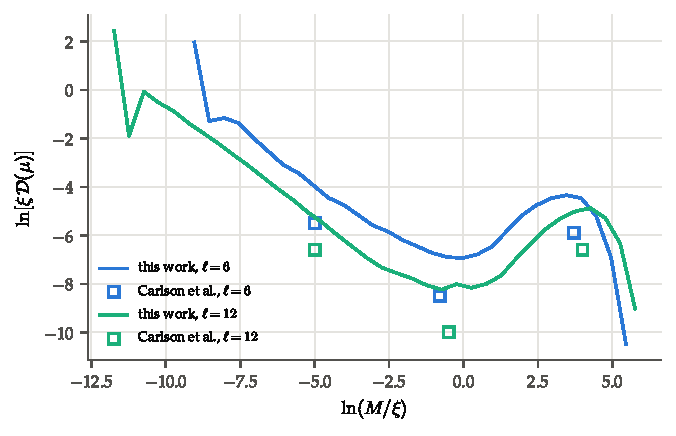
\includegraphics[width=0.62\linewidth]{results/normalisation.pdf}
  \caption{Our distributions for $\alpha=3$, $\sigma=0.01$ (lines) and three landmark values read from Fig.~3 of Carlson \emph{et al.} (1991)
  (squares).}
  \label{fig:normalisation}
\end{figure}

% ======================================================================
\section{Is the model critical? The role of \texorpdfstring{$\sigma$}{sigma}}
\label{sec:res-sigma}

\subsection{The hypothesis}

Carlson \emph{et al.} identify the friction drop $\sigma$ as the critical parameter of the 1991 model: the localization length
$\tilde\xi = (2\xi/\alpha)\ln(4\ell^2/\sigma)$ (\cref{eq:xi-tilde}) diverges as $\sigma\to0$, so that in this limit the range of localized events would
become infinite, as at a critical point. At the same time, their estimate of the crossover moment, $\tilde M = 2\xi/\alpha$, does not depend on $\sigma$.
To test this picture we simulated the model with $\alpha=3$, $\ell=6$, $N=4096$ and $\sigma$ from 0.1 down to 0.0003, each over 1000 units of plate
displacement.

\subsection{Results}

\Cref{fig:sigma} and \cref{tab:sigma} show the results. Two things are clear.

\emph{The small events depend on $\sigma$.} The one-block moment $M_1$ is proportional to $\sigma$, and as $\sigma$ decreases the distribution extends to ever
smaller moments, with the peaks of one- and few-block events moving with it (left panel). These microscopic events make the effective exponent oscillate
in the lower part of the range (middle panel).

\emph{Everything else does not.} For $\sigma\le0.03$ the distributions of moments coincide for $M\gtrsim0.03\,\xi$, and the distributions of the number of
blocks per event coincide for events of more than about ten blocks (right panel). The rate of events with ten or more blocks, the position of the minimum
of $\mathcal D(\mu)$ ($M\approx0.85\,\xi$), the position $\Delta_{\min}$ of the minimum of the block-number distribution, and the upper cutoff of the delocalized
events are all independent of $\sigma$ within the accuracy of the data. In particular, $\Delta_{\min}$ stays between 45 and 57 blocks without any trend, while the prediction for
$\tilde\xi$ grows from 34 to 52.

\begin{figure}[t]
  \centering
  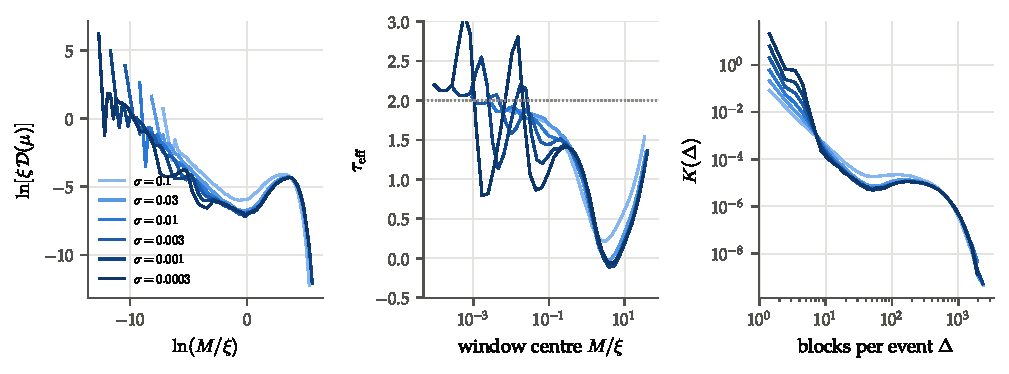
\includegraphics[width=\linewidth]{results/sigma_scan.pdf}
  \caption{The role of the friction drop $\sigma$ ($\alpha=3$, $\ell=6$, $N=4096$). Left: size distributions. Middle: effective exponent of the moment
  density in windows $[M,10M]$. Right: distribution of the number of blocks per event, per unit plate displacement and unit length.}
  \label{fig:sigma}
\end{figure}

\begin{table}[t]
\centering
\caption{Dependence on $\sigma$ ($\alpha=3$, $\ell=6$). $M_1$: one-block moment; $r_{10}$: events with at least ten blocks per block and per unit plate
displacement; $M_{\min}$: minimum of $\mathcal D(\mu)$; $\Delta_{\min}$: minimum of the block-number distribution; $\tilde\xi$: prediction
\cref{eq:xi-tilde}; $M^*$: 99th percentile of the delocalized events.}
\label{tab:sigma}
\begin{tabular}{ccccccc}
\toprule
$\sigma$ & $M_1$ & $r_{10}$ & $M_{\min}/\xi$ & $\Delta_{\min}$ & $\tilde\xi/a$ & $M^*/\tilde M$ \\
\midrule
\tabinput{figures/results/sigma_table.tex}
\bottomrule
\end{tabular}
\end{table}

\subsection{Interpretation}

The friction drop $\sigma$ controls only how small events can be; it does not control a length that grows as $\sigma\to0$. The statistics of all events of
more than a few blocks, localized and delocalized, are independent of $\sigma$ over the range studied, and no growing localization length is visible. In the
sense of \cref{sec:critical}, $\sigma$ is therefore not a critical parameter of the large-event statistics: making it smaller does not bring the model closer to
a scale-free state; it only adds microscopic events at the bottom of the distribution.

This also qualifies the ``Gutenberg--Richter'' scaling region of Carlson \emph{et al.} At $\sigma = 0.01$ the region with $b\approx1$ lies where the
$\sigma$-dependent few-block events overlap with the $\sigma$-independent localized events. Its effective exponent is not a property of the localized events
alone, and it shifts when $\sigma$ changes.

% ======================================================================
\section{Towards the continuum limit: the role of \texorpdfstring{$\ell$}{l}}
\label{sec:res-ell}

The other natural limit is $\ell\to\infty$ at fixed $\sigma$: the stiffness length $\xi=\ell a$ becomes large compared with the block spacing, and the chain
approaches the continuum equation \cref{eq:bk-cont}. Carlson \emph{et al.} argue that real faults have $\ell\sim100$. We extended their range $\ell = 6$--12 to
$\ell = 16$ and 24, with chains long enough that the largest events stay well below the system size (\cref{tab:ell}). Doubling the chain at $\ell=12$ (from 8192 to
16384 blocks) changes the upper cutoff by about 6\%, which shows that the runs at $\ell\le12$ are only marginally affected by the system size.

\begin{figure}[t]
  \centering
  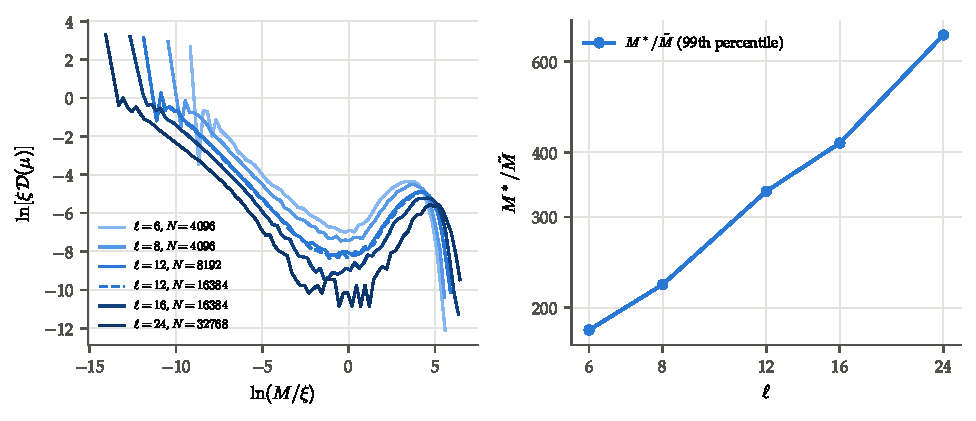
\includegraphics[width=\linewidth]{results/ell_scan.pdf}
  \caption{Approaching the continuum limit ($\alpha=3$, $\sigma=0.01$). Left: size distributions for $\ell$ from 6 to 24. Right: upper cutoff of the delocalized
  events, in units of $\tilde M = 2\xi/\alpha$.}
  \label{fig:ell}
\end{figure}

\begin{table}[t]
\centering
\caption{Dependence on $\ell$ ($\alpha=3$, $\sigma=0.01$): number of blocks, largest event (blocks), upper cutoff $M^*/\tilde M$, and the exponent of the localized
region from a maximum-likelihood fit between $\max(10M_1,10^{-4}\xi)$ and $10^{-2}\xi$.}
\label{tab:ell}
\begin{tabular}{ccccc}
\toprule
$\ell$ & $N$ & largest event & $M^*/\tilde M$ & $\tau$ \\
\midrule
\tabinput{figures/results/ell_table.tex}
\bottomrule
\end{tabular}
\end{table}

Two trends are visible (\cref{fig:ell}). First, the ratio of the upper cutoff of the delocalized events to the crossover moment grows with $\ell$, as
$M^*/\tilde M\propto\ell^{\resMstarExp}$, consistent with the rough proportionality to $\ell$ reported by Carlson \emph{et al.} The range of great events,
measured in units of the crossover, therefore grows without bound in the continuum limit. Because this ratio depends on $\ell = \xi/a$ and not on $\xi$ alone,
the block spacing remains relevant: as Carlson \emph{et al.} noted, the model has no simple continuum limit. Second, the window of the localized power law widens
(its lower end, $M_1/\xi\propto\sigma/\ell^3$, moves down), while its exponent decreases slowly, from $\tau = \restauEllG$ at $\ell=6$ to $\restauEllCE$ at $\ell=24$
($b$ from 0.96 to 0.87). Whether the exponent converges to a limiting value as $\ell\to\infty$ cannot be decided from this range.

% ======================================================================
\section{The 1989 model}
\label{sec:res-1989}

\subsection{Set-up}

The first study of Carlson and Langer~\cite{CarlsonLanger1989} used the symmetric friction law \cref{eq:phi89}, a finite loading speed $\nu$,
$\ell = 10$, and chains of 100 or 400 blocks. Their Fig.~6 shows distributions for five parameter sets, each obtained from one run of a given
length $T$ in loading periods $2/\nu$. We simulated each parameter set in two ways: as one long run, 4 to 44 times longer than theirs, and as five
independent runs of exactly their length. Events are space--time connected clusters of slip (\cref{sec:num-bk}); as in their analysis, each return
of a block's velocity to zero ends its slip episode, so that the small oscillating slips of a slowly creeping block count as separate one-block events.
With a finite loading speed the natural frequency of events is $\mathcal R(\mu)$, the number per unit time and unit length.

\subsection{Results}

\Cref{fig:cl1989} shows the distributions. All the features of their Fig.~6 are present. The tallest peak is that of one-block events, at the
magnitude $\mu_1 = \ln[2\pi\nu(2\ell^2)^{-3/2}]$ predicted by their small-event analysis ($-10.7$ for $\nu=0.01$ and $-13.0$ for $\nu=0.001$), followed by
peaks of few-block events. Then comes a straight scaling region, a minimum near $\mu\approx0$--1, and a peak of great events just below the largest
possible magnitude $\mu_L = \ln(2N)$ (dotted lines). For $\alpha=1$ (panel d) the scaling region is much flatter and the great events are weak, and for
$N=400$ (panel c) the peak of great events is lower and broader than for $N = 100$, both as in their figure.

\begin{figure}[t]
  \centering
  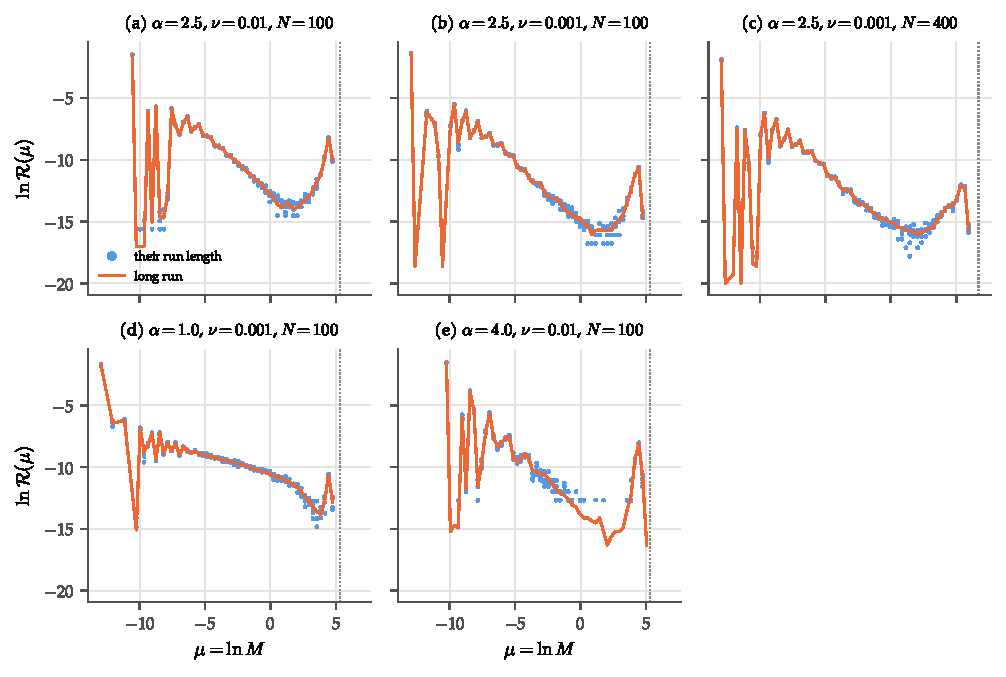
\includegraphics[width=\linewidth]{results/cl1989.pdf}
  \caption{The 1989 model with the parameters of Fig.~6 of Carlson and Langer ($\ell = 10$). Points: five independent runs of their length; line: one long
  run. Dotted line: $\mu_L=\ln(2N)$.}
  \label{fig:cl1989}
\end{figure}

\Cref{tab:cl1989} gives the exponent $b$ of the scaling region, from maximum-likelihood fits in $e^{-5}<M<e^{-1}$ ($e^{-7}<M<e^{2}$ for $\alpha=1$).
For $\alpha = 2.5$ we find $b = 0.89$--$0.94$, and for $\alpha = 1$, $b=0.29$, in reasonable agreement with their values $b\approx1$ and $b\approx0.35$
(their Fig.~7). For $\alpha=4$ we find $b = 0.80$, whereas their Fig.~7 gives $b\approx1$ for all $\alpha\ge2.5$.

\begin{table}[t]
\centering
\caption{The 1989 model: exponent $b$ of the scaling region from one long run, and its range over five independent runs of the original length $T$
(in loading periods).}
\label{tab:cl1989}
\begin{tabular}{cccccc c}
\toprule
 & $\alpha$ & $\nu$ & $N$ & $T$ & $b$ (long run) & $b$ (runs of length $T$) \\
\midrule
\tabinput{figures/results/cl1989_table.tex}
\bottomrule
\end{tabular}
\end{table}

\subsection{How much data did the 1989 study need?}

The five independent runs of the original length show how precisely the published distributions could be determined. For panels (a)--(d) the
small and intermediate events are well determined at the original length, and the spread of $b$ between runs is a few hundredths. The great events
are a different matter: they occur roughly once per loading period, so a run of 45 or 50 loading periods (panels d and e) contains only a few dozen of
them, and their part of the distribution differs visibly from run to run. For $\alpha = 4$ (panel e) even the exponent of the scaling region varies between
0.71 and 0.90 among runs of the original length, so their value $b\approx1$ at large $\alpha$ is within the statistical uncertainty of a single short run but
is not confirmed by our long run. This supports the suspicion, raised at the beginning of this project, that some of the published distributions were based
on too little data.

The main obstacle to reproducing the 1989 paper in the earlier version of this project was, however, not the length of the runs but the implementation
(\cref{sec:num-legacy}) and the definition of events. With a finite loading speed, slip somewhere in the chain is almost never absent, and defining an event as
``everything between two quiet periods'' merges unrelated slips into a few huge events; the space--time cluster definition, with each zero of a block's
velocity ending its episode, is needed to recover the distributions of Carlson and Langer.

% ======================================================================
\section{Summary: is the Burridge--Knopoff model critical?}
\label{sec:res-summary}

The results of this chapter and of Chapter~\ref{ch:mapping} answer the question in several parts.
\begin{enumerate}
  \item \textbf{There are power laws.} Localized events follow a power law with $b\approx0.9$ ($\tau\approx1.9$) for strong velocity weakening and
    $b\approx0.3$--$0.4$ for $\alpha=1$, over one to several decades in moment, in both the 1989 and the 1991 versions of the model.
  \item \textbf{Their range is set by the model, not by the system size.} The localized power law ends at a crossover moment $\tilde M\approx\xi$, and the
    great events have a cutoff $M^*\propto\ell^{\resMstarExp}\tilde M$; once the chain is several times longer than the largest event, the distributions no longer
    depend on its length. In SOC proper, by contrast, the only cutoff is the system size.
  \item \textbf{The friction drop $\sigma$ is not a critical parameter.} Reducing $\sigma$ by a factor of 100 (from 0.03 to 0.0003) changes only the smallest events; the statistics of all events
    of more than a few blocks, and the crossover length, stay the same.
  \item \textbf{The continuum limit $\ell\to\infty$ widens the windows.} Both the localized power law and the range of great events grow with $\ell$, while the exponent
    of the localized region drifts slowly ($\tau$ from 1.96 to 1.87 between $\ell = 6$ and 24). The block spacing remains relevant, so the model has no simple continuum
    limit.
  \item \textbf{The great events are characteristic, not critical.} They form a separate population with a peak and a sharp cutoff, which is the opposite of scale
    invariance, and they are produced by the inertial amplification of slip that the sandpile limit lacks (Chapter~\ref{ch:mapping}).
\end{enumerate}
The one-dimensional Burridge--Knopoff model is therefore not self-organized critical in the strict sense. It produces Gutenberg--Richter-like statistics over a window
bounded below by the microscopic events and above by a crossover set by the stiffness length, together with an excess of characteristic great events. The parameter that
controls how wide this window is, is the stiffness ratio $\ell$, i.e.\ the separation between the block spacing and the stiffness length, and not the friction drop or the
loading speed.
